\chapter{Prediction Filters}
\label{ch:part3}

I dette kapitel vil vi vise at man kan fremstille filtre, der kan reducere memory i signaler, og derved kunne bruge færre bits til at quantize signalet. Dette omtales ofte i litteraturen som Linear Predictive Coding.

\section{Spørgsmål A + B - LPC Coding}

LPC anvender en række af de foregående samples, til at lineært forudsige (eng.: predict) den næste sample. En god forudsigelse giver en lille difference mellem den originale sample, og den forudsagte sample. Denne fejl eller difference har en mindre dynamisk range, og kan derfor quantiseres med færre bits end det originale signal. Dette giver en væsentlig kompression af det transmitterede signal, da kun fejlen mellem samples skal transmitteres.

Det forudsagte signal $\tilde{x}[n]$ ud fra det orignale signal $x[n]$, har fejlen $\epsilon[n]$. Ligning \ref{eq:part3_1} og figur \ref{fig:part3_x1} beskriver sammenhængen mellem det originale signal, det predictede signale og fejlen.

\begin{figure}[!ht]
	\centering
	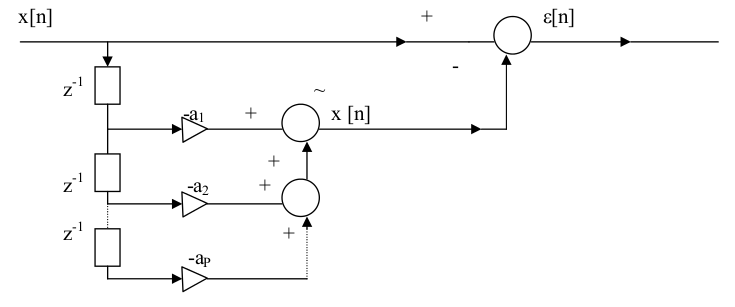
\includegraphics[width=0.8\textwidth]{resources/part3_block}
 	\caption{Blok-diagram}
 	\label{fig:part3_x1}
\end{figure}

\begin{equation}\label{eq:part3_1}
	\tilde{x}[n] = \sum^P_{i=1} a_i x[n-i] = h[h] * x[n] \Rightarrow \epsilon[n] = x[n] - \tilde{x}[n] = \sum^P_{i=0} x[n-1], a_0 = 1
\end{equation}

\subsection{Simpelt 2-tap prediction filter}
For at lave et 2-tap prediction skal vi kende en række ting:

\begin{itemize}
	\item L: Antal samples der skal bruges til at finde a-koefficienterne. Det er vigtigt at signalet er stationært i hele perioden. For et 8 kHz tale-signal, dette er omkring 20 ms, hvilket er 160 samples.
	\item Signal space: En vektor $(x[0],x[1],...,x[L-1])^{transposed}$
	\item Performance funktion: $J(a_1, a_2)$ \\
	Funktionen er defineret som summen af fejl mellem output og referencen kvadreret (dvs energien i fejlen).
	\begin{equation}
		J(a_1,a_2) = \sum^{L-1}_{k=0} | x[k] - \tilde{x}[k] |^2
	\end{equation}
	Ved et 2-tap filter, denne summation kan udvides til
	\begin{equation}
		\begin{aligned}
		J(a_1,a_2) &= \sum^{L-1}_{n=0} | x[n] + a_1 x[n-1] + a_2 x[n-2] |^2 \\
		&= \sum^{L-1}_{n=0} ( x[n]^2 + a_1^2 x[n-1]^2 + a_2^2 x[n-2]^2 \\ 
		& + 2a_1 a_2 x[n-1] x[n-2] + 2a_1 x[n] x[n-1] + 2a_2 x[n]x[n-2])
		\end{aligned}
	\end{equation}

	Det er værd at nævne, at performance funktionen aldrig er negativ, samt at den (næsten) altid vil være $> 0$. For at finde minimum for funktion har vi brug for at løse

	\begin{equation}
		\frac{\partial J}{\partial a_1} = \frac{\partial J}{\partial a_2} = 0
	\end{equation} 

	For at finde koefficienterne for et 2-tap filter, kan følgende ligningssystem opstilles

	\begin{equation}
		\begin{aligned}
			\left\{ \sum^{L-1}_{n=0}x[n-1]^2 \right\} a_1 + \left\{ \sum^{L-1}_{n=0} x[n-1]x[n-2]\right\} a_2 &= -\sum^{L-1}_{n=0}x[n]x[n-1] \\
			\left\{ \sum^{L-1}_{n=0} x[n-1]x[n-2] \right\} a_1 + \left\{ \sum^{L-1}_{n=0} x[n-2]^2 \right\} a^2 &= -\sum^{L-1}_{n=0}x[n]x[n-2]
		\end{aligned}
	\end{equation}

	Hvis $r_{xx}[m]$ er autocorrelations-funktionen for det samplede signal $x[n]$, $p$ er antallet af taps, kan ligningerne opskrives på den mere generalle form

	\begin{equation}
		\sum^p_{i=1} a_i r_{xx}[i-j] = r_{xx}[j] \text{ , hvor } j = 1,2,...,p
	\end{equation}

	Dette kan også skrives i matrix form, som forsimpler det endnu mere. $\mathbf{R}$ er autocorrelations-matricen, $\mathbf{a}$ er koefficientsvektoren og $\mathbf{r}$ er autocorrelations-vektoren.

	\begin{equation}\label{eq:part3_7}
		\mathbf{Ra} = \mathbf{r} \Rightarrow \mathbf{a} = \mathbf{R^{-1} r}
	\end{equation}
\end{itemize}


Alt dette kan realiseres i MATLAB, hvor vi samtidig kan efterprøve resultatet ved at sammenligne med MATLABs indbyggede lpc function. Listing \ref{lst:part3_1} viser MATLAB-koden til vores første eksperiment. Først laves en Markov kæde med to tilstande, hvor der genereres 100 samples. Herefter udregnes autocorrelationen for signalet, og koefficienter udregnes ved hjælp af matrice-ligningen givet i ligning \ref{eq:part3_7}. Til sidst udregnes koefficienterne ved hjælp af MATLABs lpc funktion, for at sammenligne. Bemærk at $r_{xx}[m]$ er $rr(100 + m)$ i MATLAB-koden.

Ved en kørsel (se listing \ref{lst:part3_2}) kan vi se at vores egen udregning passer. 

\lstset{language=MATLAB,numbers=left}
\begin{figure}
	\begin{lstlisting}[frame=single, caption=Udregning af LPC koefficienter,label=lst:part3_1]
N = 100;
tt = [0.7, 0.3; 0.4, 0.6];

yy = markov2st(tt, N);
yy = yy - mean(yy);

rr = xcorr(yy);

R = [rr(100) rr(101); rr(101) rr(100)];
r = -[rr(101); rr(102)];

my_a = inv(R) * r
lpc_a = lpc(yy, 2)

error = filter(real([1, my_a]),1,yy);
PG = 10*log10(var(yy)/var(error))
	\end{lstlisting}
\end{figure}


\lstset{language=MATLAB,numbers=left}
\begin{figure}
	\begin{lstlisting}[frame=single, caption=Udregning af LPC koefficienter - output,label=lst:part3_2]
my_a =
    -0.3249    0.0322

lpc_a =
    1.0000   -0.3249    0.0322

PG = 10.0002
	\end{lstlisting}
\end{figure}

Ud fra det originale signal og fejlen ved prediction filteret, kan vi udregne en såkaldt Prediction Gain, som beskriver forholdet mellem størrelsen af det originale signal og størrelsen af fejlen. I listing \ref{lst:part3_2} kan vi se at vi opnår en prediction gain på lidt over $10\ dB$.

Figur \ref{fig:part3_1} viser et stem af signalet, og figur \ref{fig:part3_2} viser et stem af fejlen. Her er det altså tydeligt at det dynamiske range er drastisk formindsket.

\begin{figure}[!ht]
	\centering
	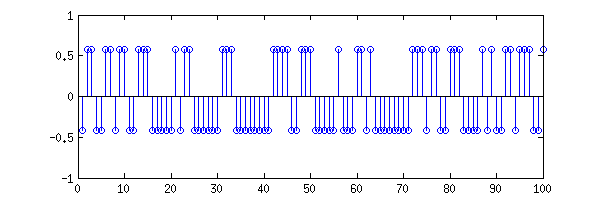
\includegraphics[width=0.8\textwidth]{resources/part3_signal}
 	\caption{Stem af signalet}
 	\label{fig:part3_1}
\end{figure}

\begin{figure}[!ht]
	\centering
	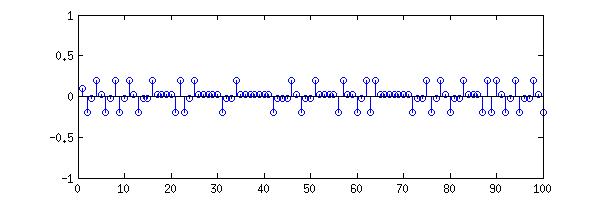
\includegraphics[width=0.8\textwidth]{resources/part3_error}
 	\caption{Stem af fejlen}
 	\label{fig:part3_2}
\end{figure}


\section{Spørgsmål C + D}

I dette spørgsmål generere vi et signalet med `white noise`, ved hjælp af MATLAB's `randn` funktion. Formålet er herefter at tilføje memory til dette signal ved at lavpas-filtrere det, for derefter at fjerne støjen igen ved hjælp af et LPC filter.

Figur \ref{fig:part3_3} viser auto-correlation af white noise signalet. Her er det tydeligt at signalet ikke indeholder memory. For at tilføje memory har vi lavet et lavpas-filter (ved hjælp faf MATLAB's fdatool), med følgende egenskaber: 

\begin{itemize}
	\item $f_s = 48000\ Hz$
	\item $f_{pass} = 12000\ Hz$
	\item $f_{stop} = 9600\ Hz$
	\item Orden: 12
\end{itemize} 

\begin{figure}[!ht]
	\centering
	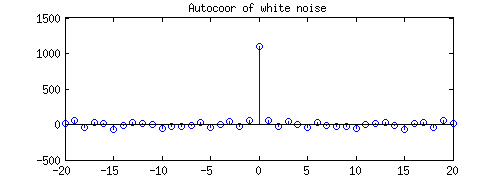
\includegraphics[width=0.8\textwidth]{resources/part3_white_noise_xcorr}
 	\caption{Stem af auto-correlationen af white noise}
 	\label{fig:part3_3}
\end{figure}

Ved af filtrere white noise-signalet med lavpas-filteret, tilføjer vi memory til signalet. Dette kan tydeligt ses på auto-correlationen på figur \ref{fig:part3_4}. Selve frekvensresponsen for LP-filteret kan ses på figur \ref{fig:part3_5}.

\begin{figure}[!ht]
	\centering
	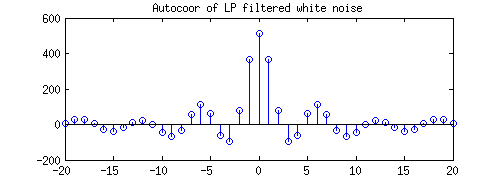
\includegraphics[width=0.8\textwidth]{resources/part3_lp_filtered_white_noise_xcorr}
 	\caption{Stem af auto-correlationen af LP-filtreret white noise}
 	\label{fig:part3_4}
\end{figure}

For at fjerne det memory som er blevet tilføjet, kommer LPC filteret ind i billedet. Dette kaldes også for et whitening filter, da det giver signalets dets white noise karakteristik tilbage. Da LP-filteret er et 12. ordens filter, har vi også lavet et 12. ordens LPC-filter. Koefficienter findes ved hjælp af MATLAB's `lpc`, hvorefter error signalet udregnes ved hjælp af MATLAB's `filter`. Det resulterende signal's auto-correlation er plottet på figur \ref{fig:part3_6}. Her kan det ses at stort set alt memory er forsvundet - LPC-filteret har altså virket efter hensigten, og fjernet memory fra signalet. Frekvensresponsen for LPC-filteret kan ses på figur \ref{fig:part3_5}. Den grønne linje på figur \ref{fig:part3_5} viser den summerede frekvensrespons for de to filtre. Hvis begge systemer of filtre var ideelle, skulle LPC-filteret gerne udhviske LP-filterets virkning, og gen grønne linje burde ligge på præcis 0 dB (forstærkning på 1). 

\begin{figure}[!ht]
	\centering
	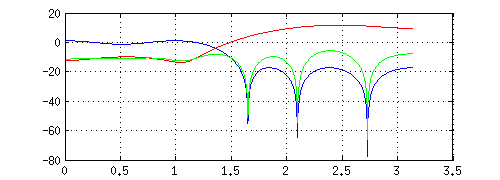
\includegraphics[width=0.8\textwidth]{resources/part3_lp_and_whitening_filter}
 	\caption{Frekvensresponse for LP (blå), whitening filter (rød) og summen af de to filtre (grøn)}
 	\label{fig:part3_5}
\end{figure}

\begin{figure}[!ht]
	\centering
	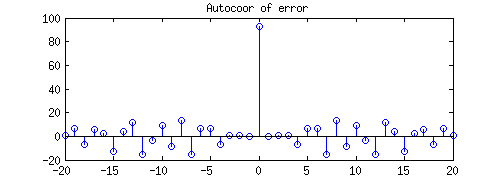
\includegraphics[width=0.8\textwidth]{resources/part3_error_xcorr}
 	\caption{Stem af auto-correlationen af error}
 	\label{fig:part3_6}
\end{figure}

\begin{figure}[!ht]
	\centering
	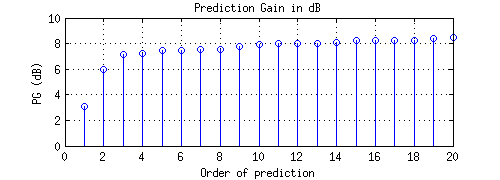
\includegraphics[width=0.8\textwidth]{resources/part3_pg_as_function_of_order}
 	\caption{Plot af prediction gain som funktion af LPC-filterets orden}
 	\label{fig:part3_7}
\end{figure}

Figur \ref{fig:part3_7} viser et plot af LPC-filterets prediction gain, som function af filterets orden. Ud fra dette plot, kan det ses at prediction gain stiger mest fra 2. orden of til 4. orden, hvorefter det stiger langsomt op til 10. orden, for derefter at flade helt ud.


